% Contributions are much appreciated, in order to contribute to this project, head over to this repository:
% https://github.com/bshramin/uofa-eng-assignment

\documentclass[11pt,letterpaper]{article}
\textwidth 6.5in
\textheight 9.in
\oddsidemargin 0in
\headheight 0in
\usepackage{graphicx}
\usepackage{fancybox}
\usepackage[utf8]{inputenc}
\usepackage{epsfig,graphicx}
\usepackage{multicol,pst-plot}
\usepackage{pstricks}
\usepackage{amsmath}
\usepackage{amsfonts}
\usepackage{amssymb}
\usepackage{eucal}
\usepackage[left=2cm,right=2cm,top=2cm,bottom=2cm]{geometry}
\usepackage{esvect}
\pagestyle{empty}
\DeclareMathOperator{\tr}{Tr}
\newcommand*{\op}[1]{\check{\mathbf#1}}
\newcommand{\bra}[1]{\langle #1 |}
\newcommand{\ket}[1]{| #1 \rangle}
\newcommand{\braket}[2]{\langle #1 | #2 \rangle}
\newcommand{\mean}[1]{\langle #1 \rangle}
\newcommand{\opvec}[1]{\check{\vec #1}}
\renewcommand{\sp}[1]{$${\begin{split}#1\end{split}}$$}

\usepackage{lipsum}

\usepackage{listings}
\usepackage{color}
\usepackage{wrapfig}
\usepackage[shortlabels]{enumitem}

\definecolor{codegreen}{rgb}{0,0.6,0}
\definecolor{codegray}{rgb}{0.5,0.5,0.5}
\definecolor{codepurple}{rgb}{0.58,0,0.82}
\definecolor{backcolour}{rgb}{0.95,0.95,0.92}

\lstdefinestyle{mystyle}{
	backgroundcolor=\color{backcolour},   
	commentstyle=\color{codegreen},
	keywordstyle=\color{magenta},
	numberstyle=\tiny\color{codegray},
	stringstyle=\color{codepurple},
	basicstyle=\footnotesize,
	breakatwhitespace=false,         
	breaklines=true,                 
	captionpos=b,                    
	keepspaces=true,                 
	numbers=left,                    
	numbersep=5pt,                  
	showspaces=false,                
	showstringspaces=false,
	showtabs=false,                  
	tabsize=2
}

\lstset{style=mystyle}

\begin{document}
\pagestyle{plain}

\begin{flushleft}
Estudiante: Fabio Quimbay\\
Email: fabio.quimbay883@comunidadunir.net\\
Profesor: Miguel Ángel Cabeza\\
Fecha: Noviembre 7 de 2022\\
\end{flushleft}

\begin{flushright}\vspace{-20mm}

\includegraphics[height=2cm]{logo.png}
\end{flushright}
 
\begin{center}\vspace{0cm}
\textbf{\large PER5786 2022-2023  Física 1 (GFI) - PER5786 2022-2023}\\
 Tema 2 - Cinemática
\end{center}

 
\rule{\linewidth}{0.1mm}
%%%%%%%%%%%%%%%%%%%%%%%%%%%%%%%%%%%%%%%%%%%%%%%%%%%%%%%%%%%%%%%%%%%%%%%%

\bigskip
\bigskip

%%%%%%%%%%%%%%%%%%%%
\textbf{Ejercicio 4 propuesto}\\

\begin{wrapfigure}{r}{0.25\textwidth}
    \centering
    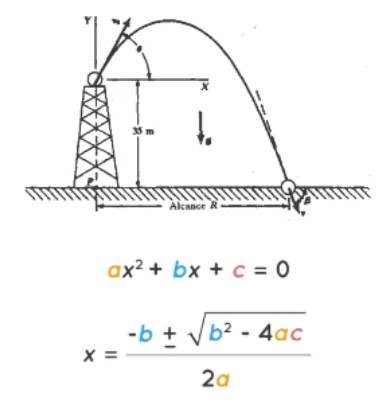
\includegraphics[width=0.25\textwidth]{ejemplo_4.png}
\end{wrapfigure}

Un objeto es arrojado hacia arriba desde la azotea de una torre de 35 m, con velocidad inicial $v0 = 80 m/s$ y un ángulo $\theta = 25^\circ$. Datos: aceleración gravitatoria terrestre $g = 9.8 m/s^2$.

\begin{enumerate}[(a)] 
\item {Encuentra el tiempo que tarda en llegar al suelo, y el alcance, es decir, la distancia R desde la base de la torre, P, al punto de impacto.}
\item {Calcula la magnitud y el ángulo $\beta$ de la dirección de la velocidad en el momento del impacto.}
\end{enumerate}

\textbf{Formulas base:}\\

Se tomarán las siguientes formulas base:\\

\textbf{Movimiento horizontal}\\

\begin{align}
\boxed{ r_{x} = \vec{V_{0_{x}} \cdot t}}\\
\boxed{ v_{x} = \vec{V_{0_{x}}}}
\end{align}

\textbf{Movimiento vertical}\\

\begin{align}
\boxed{ r_{y} = r_{0}y + \vec{V_{0_{y}}} \cdot t + 1/2 \cdot g \cdot t^2}\\
\boxed{ v_{y} = \vec{V_{0_{x}}} + g \cdot t}
\end{align}


\textbf{Solución:}\\

\textbf{a)}: Tiempo que tarda en llegar al suelo, y el alcance, es decir, la distancia R desde la base de la torre, P, al punto de impacto; primero es necesario determinar las componentes de la $\vec{V_{0}}$ a saber:

\begin{align}
\boxed{ \vec{V_{0_{x}}} = |\vec{V_{0}}| \cdot cos \alpha}\\
\boxed{ \vec{V_{0_{y}}} = |\vec{V_{0}}| \cdot sin \alpha}
\end{align}

Con esta información ahora se puede determinar el tiempo en llegar al suelo (altura será igual a $0$), a través de las raices del polinómio,así:

\begin{align*}
	r_{y} &= r_{0}y + \vec{V_{0_{y}}} \cdot t + 1/2 \cdot g \cdot t^2\\
	0 &= 35 + 33.8095 - 4.9 \cdot t^2\\
	roots &= \{ t_{1}: -0.914109\,s, t_{2}: 7.81401\,s \}
\end{align*}

El tiempo en llegar al suelo es de $\textbf{7.81401\,s}$.\\

La distancia horizontal viene dada por la siguiente formula:

\begin{align*}
	d_{HOR} &= \vec{V_{0_{x}}} \cdot t \\
	d_{HOR} &= 72.5046 \cdot 7.81401 \\
	d_{HOR} &= 566.52 m
\end{align*}

La distancia horizontal a la que llega el objeto es de $\textbf{566.52\,m}$.\\

\textbf{b)}: Magnitud y el ángulo $\beta$ de la dirección de la velocidad en el momento del impacto, a saber:

\begin{align*}
	V_{f_{x}} &= V_{0_{x}}\\
	V_{f_{x}} &= 72.5946\, m/s\\
	V_{f_{y}} &= V_{0_{y}} + g \cdot t\\
	\,\\
	V_{f_{y}} &= 33.8095 + 4.9 \cdot 7.814\\
	V_{f_{y}} &= -42.7677\,m/s
	\,\\ \,\\
	tan \beta &= \frac {V_{f_{y}}}{V_{f_{x}}} = \frac {-42.7677}{72.5946}\\ \,\\
	\beta &= arctan \frac {-42.7677}{72.5946}\\
	\beta &= -30.5347 ^\circ
\end{align*}

La magnitud y el ángulo en P, cuando el objeto llega al suelo es de $\textbf{\{72.5046, -42.7677\}\,m/s}$ y $\textbf{-30.5347}$$^\circ$, respectivamente.\\

%%%%%%%%%%%%%%%%%%%%

\end{document}

